\chapter{Multi-layer Kernel Machines}
\label{chap_mkm}
%This chapter introduces the concept of MKMs proposed in \cite{saul} et al., followed by an empirical study on some popular datasets cited extensively in deep learning literatures. This chapter is organized as follows; section \ref{chap2_mkm} gives a brief introduction to MKMs and the multi-layer composition of few kernel functions, section \ref{chap2_exp} contains the results of empirical study using MKMs, section \ref{chap2_tsne} talks about the visualization technique used to plot the distribution of digits(from \cite{mnist} dataset) in a low-dimensional space, section \ref{chap2_mkm_mix} contains the results of empirical study on MKMs with mixed kernels and section \ref{chap2_conc} concludes the chapter.  


%\label{chap2_mkm}
Multi-layer Kernel Machines (MKMs\nomenclature{MKM}{Multi-layer Kernel Machines}) were first introduced by \cite{saul} et al. In their framework, arc-cosine kernel  which itself is having a layered architecture was used. The architecture of MKMs consists of $L$ layers and in each layer the data is subjected to unsupervised dimensionality reduction methods, viz. kernel PCA(\cite{kpca} et al.),  followed by a supervised feature selection. 

The MKM machines use multilayer kernel function, whose description is given in the next section. The rest of the chapter is organized as follows: section \ref{chap2_exp} contains the results of empirical study using MKMs, section \ref{chap2_tsne} describes the visualization technique used to plot the distribution of digits (from \cite{mnist} dataset) in a low-dimensional space, section \ref{chap2_mkm_mix} contains the results of empirical study on MKMs with mixed kernels and  concluding remarks are given in section \ref{chap2_conc}.  

\section{Multi-layer Kernel}
Corresponding to each Reproducing kernel Hilbert spaces (RKHS) $\mathcal{F}$ there exists a unique reproducing kernel 
$k: \mathcal{X} \times \mathcal{X} \rightarrow \mathcal{F}$,  where $ k(x,y) = \phi(x) \cdot \phi(y), x, y \in \mathcal{X} \; \text{where} \; \mathcal{X}    \text{ is a normed space, } \phi(x), \phi(y) \in \mathcal{F}$ and $\cdot$ is the inner product defined on $\mathcal{F}$.

Iteratively applying the mapping $\phi(\cdot)$ on the inputs $x \textrm{ and } y$ and then taking their inner product, we can obtain an L-layer kernel function as
\[ k^{(L)}(x,y) = \underbrace{\phi(\phi(\ldots \phi(x)))}_{\textrm{L times}} \textrm{ } \cdot \textrm{ } \underbrace{\phi(\phi(\ldots \phi(y)))}_{\textrm{L times}} \]

Thus a $L$ layer kernel machine consists of $L$ RKHS's.

\subsection{Multi-layer Composition of Polynomial and Gaussian Kernels}
\label{chap2_mlother}
A polynomial kernel of degree d is defined as follows
\[k(x, y) = (x \cdot y)^d\]
Consider a two layer composition of polynomial kernel which can be computed as
\begin{equation*}
\begin{aligned}
\phi(\phi(x)) \cdot \phi(\phi(y)) &= \bigg(\phi(x) \cdot \phi(y)\bigg)^d \\
& = {(x \cdot y)^d}^d =  {(x \cdot y)^d}^2 
\end{aligned}
\end{equation*}
Thus the higher order compositions of polynomial kernels are simply polynomials of higher degree than the one from which it is constructed.

The two layer composition for gaussian kernels $k(x, y) = e^{-\lambda\norm{x-y}^2} $ is given by
\begin{equation*}
\begin{aligned}
\phi(\phi(x)) \cdot \phi(\phi(y)) &= e^{-\lambda\norm{\phi(x)-\phi(y)}^2} \\
& = e^{-2\lambda(1-k(x, y))}
\end{aligned}
\end{equation*}

\subsection{Multi-layer Composition of Arc-cosine Kernels}
\label{chap2_mlarc}
Let x, y be two inputs in $\mathbb{R}^d$. Define $\theta$ as the angle between them.
\[ \theta = cos^{-1}\left ( \frac{x\cdot y}{\left \| x \right \| \left \| y \right \|} \right ) \]
Then the kernel function computed by the arc-cosine kernel is
\begin{equation}
k_n(x,y) = \frac{1}{\pi}\left \| x \right \|^n \left \| y \right \|^n J_n(\theta)
\label{arc_cosine_kernel} 
\end{equation}
where n is called the \textit{degree of the kernel} and
\[ J_n(\theta) = (-1)^n(sin\theta)^{2n+1} \left ( \frac{1}{sin\theta} \frac{\partial}{\partial \theta} \right )^n \left ( \frac{\pi-\theta}{sin\theta} \right ) \]

$J_n(\theta)$ for n=0, 1, 2 is computed as shown below.
\[ J_0(\theta) = \pi-\theta \]
\[ J_1(\theta) = sin\theta + (\pi-\theta)cos\theta \]
\[ J_2(\theta) = 3sin\theta cos\theta + (\pi-\theta)(1+2cos^2\theta) \]
for n=0, it takes the simple form
\[k_0(x,y) =  1- \frac{1}{\pi}cos^{-1}\left ( \frac{x\cdot y}{\left \| x \right \| \left \| y \right \|} \right )  \]
hence the name arc-cosine kernel is given.The kernel function computed by arc-cosine kernel is related to the computation of multi-layer threshold networks as shown below.

Consider a single layer neural network with weights $W_{ij}$ that connects the $j^{th}$ input unit to the $i^{th}$ output unit(see figure \ref{fig_singnet}). The network maps input $x$ to output $f(x)$ by applying a non-linear map 
\[ f(x) = g(W \cdot x) \]
where the non-linearity is described by the network`s activation function
\[g_n(z) = \Theta(z)z^n \]
with 
\[ \Theta(z) = \frac{1}{2}(1+sign(z)) \]
this activation function is called one-sided polynomial activation function, whose graph for different n values is also shown in figure \ref{fig_singnet}.

\begin{figure}[H]
  \centering
  \captionsetup{justification=centering,margin=0.1cm}
  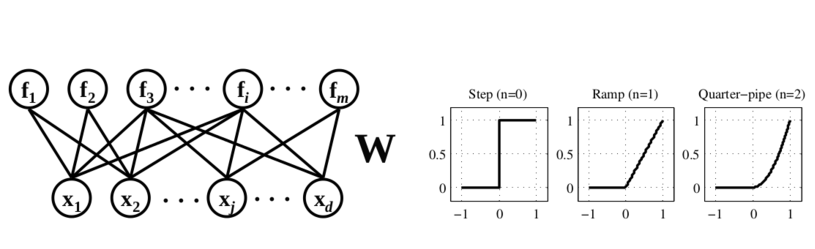
\includegraphics[width=1.0\linewidth, height=7cm]{figures/singnet}
  \caption{Single layer network and thresholded activation functions(\cite{saul} et al.)}
  \label{fig_singnet}
\end{figure}

Let $f(x)$ and $f(y)$ be the outputs corresponding to inputs $x$ and $y$. Then the inner product of $f(x)$ and $f(y)$ is
\[ f(x)\cdot f(y) = \sum_{i=1}^m \Theta(w_i\cdot x) \Theta(w_i\cdot y)(w_i\cdot x)^n (w_i\cdot y)^n\]
Here $w_i$ is the $i^{th}$ row of weight matrix $W$ and $m$ is the no of output units. Assume $W_{ij}$ are Gaussian distributed with zero mean and unit variance and the network has an infinite number of output units. Then
\[ lim_{m\rightarrow \infty} \frac{2}{m}f(x)\cdot f(y) = k_n(x,y) \]
where
\begin{equation}
k_n(x,y) = 2\int dw \frac{e^{-\frac{\norm{w}^2}{2}}}{(2\pi )^{d/2}} \Theta (w\cdot x) \Theta (w\cdot y) (w\cdot x)^n (w\cdot y)^n 
\label{arc_cosine_integral}
\end{equation}
The kernel function obtained in equation \ref{arc_cosine_integral} can be converted into an alternate form as in equation \ref{arc_cosine_kernel} with the derivation shown in \cite{saul} et al.

The multi-layer composition of arc-cosine kernel can be recursively computed as
\[ k^{(L+1)}_n(x,y) = \frac{1}{\Pi} \Bigg[ k^{(L)}(x,x) \textrm{ } k^{(L)}(y,y)\Bigg]^{\frac{n}{2}} J_n(\theta_n^{(L)}) \]
where $\theta_n^{(L)}$ is the angle between images of $x \textrm{ and } y$ in the feature space after L layer composition
\[ \theta_n^{(L)} = \textrm{cos}^{-1}\Bigg( k^{(L)}(x,y) \Bigg[ k^{(L)}(x,x) \textrm{ } k^{(L)}(y,y)\Bigg]^{\frac{-1}{2}} \Bigg) \]
In the above formulation, we have assumed that the arc-cosine kernels have the same degree $n$ at every layers of recursion. We can also use kernels of different degree at different layers. The intuition behind the multi-layer composition in case of arc-cosine kernels is, if the base kernel $k(x,y) = \phi(x) \cdot \phi(y)$ can mimic the computation of a single-layer network, then the iterated mapping in $k^{(L)}(x,y)$ can mimic the computation of multi-layer network(\cite{saul} et al.).

\subsection{MKM Architecture}
 The architecture of MKMs for solving classification tasks  is similar to that of neural network based deep learning machines, with unsupervised feature extraction(using Kernel PCA, \cite{kpca} et al.) followed by supervised feature selection in each layer. Figure \ref{fig_mkm} shows the architecture of an MKM consisting of $L$ layers of non-linear transformations.

\begin{figure}[h]
  \centering
  \captionsetup{justification=centering,margin=0.1cm}
  \includegraphics[scale=0.5]{figures/mkm}
  \caption{An MKM with L layers of transformations. Each layer consists of unsupervised feature extraction(using kernel PCA) followed by supervised feature selection.}
  \label{fig_mkm}
\end{figure}

The supervised feature selection allows us to retain only those set of features that are most informative for the pattern recognition task. The number of features to be passed to the next layer determines the width of that layer. The optimal layer width is computed by ranking the features based on their importance and selecting the required set of feature with the help of a lightweight classifier (detailed procedure is given in the experiments section). This procedure determines the architecture of the network in a greedy, layer-by-layer fashion. In their implementation \cite{saul} et al. used exhaustive search in the range 10 to 300 to determine the optimal set of features. The output from the final layer can be passed to any classifier. Though any kernel can be used for the kernel PCA based feature extraction, \cite{saul} et al. emphasized on using arc-cosine kernels due to their similarity with deep learning architecture of neural networks and the inclusion of multiple layers is significant  only in case of arc-cosine kernels.

\section{Experiments on Arc-cosine Kernel MKMs}
\label{chap2_exp}
Empirical study was conducted on four datasets, in which three were created from \cite{mnist} dataset of handwritten digits by adding noise in the background and one was a binary classification problem on shape images. The detailed experimental set up and a short description about datasets used is given below. 
\subsection{Experimental Set-Up}
In the training phase, for each layer we set apart 10000 datapoints for training the model and 2000 datapoints for cross validating kernel parameters. For the kernel PCA we chose 3000 datapoints  from the training set of 10000 images randomly. In each layer after extracting features with KPCA, we train a lightweight classifier like kNN and test the performance on the held out 2000 images. The best kernel parameter was chosen based on this performance values. With that parameter value, we did feature extraction on the entire dataset and then passed it to feature selection module. The feature selection was done by using univariate feature selection method available in \cite{scikit} library. This method produces a ranking of features with a univariate statistical test. Based on this rank we can choose the required number of important features. We chose top 5 percent features based on this rank, since empirically it was giving a consistant performance.

In the final classification stage SVMs with arc-cosine kernels are used. The metric used for comparing the performance is, percentage loss in test dataset. Percentage loss is estimated as
\[ \textrm{loss in percentage} = \Bigg(1 - \frac{\# \textrm{correct classifications}}{\# \textrm{datapoints}} \Bigg) \times 100 \]

\subsection{Mnist-back-rand Dataset}
The \textit{mnist-back-rand} dataset was created by filling the image background with random pixel values. Each pixel value of the background was generated uniformly between 0 and 255. Image size is 28$\times$28 and the dataset contains 12000 training and 50000 testing images.
\subsection{Mnist-back-image Dataset}
The \textit{mnist-back-image} dataset was generated by filling the image background with random image patches. The patches were extracted randomly from a set of 20 images downloaded from the internet. The dataset contains contains 12000 training and 50000 testing images, each of size 28$\times$28.
\subsection{Mnist-rot-back-image Dataset}
The \textit{mnist-rot-back-image} is a rotated variant of \textit{mnist-back-image} where the rotation angle is generated uniformly between $0$ and $2\pi$. Image size and number of samples are also the same as \textit{mnist-back-image} dataset.
\subsection{Rectangles-image Dataset}
For \textit{rectangles-image} dataset, the classification task is to identify whether a rectangle contained in an image has larger width or length. The dataset is constructed by uniformly sampling the height and width of the rectangles. Then random image patches are added in the background, where image patches are extracted from one of the 20 images used by \textit{mnist-back-image}. Each image is of size 28$\times$28 and each dataset contains 12000 training images and 50000 testing images.

Figure \ref{samples} contains some sample images from first three dataset and Figure \ref{chap2_rect} contains the samples from \textit{rectangles-image} dataset.
\begin{figure}[h]
  \centering
  \captionsetup{justification=centering,margin=0.1cm}
  \includegraphics[scale=0.55]{figures/data_sample1}
  \caption{sample images from \textit{mnist-back-rand}(first row), \textit{mnist-back-image}(second row) and \textit{mnist-rot-back-image}(third row) datasets.}
  \label{samples}
\end{figure}

\begin{figure}[h]
  \centering
  \captionsetup{justification=centering,margin=0.1cm}
  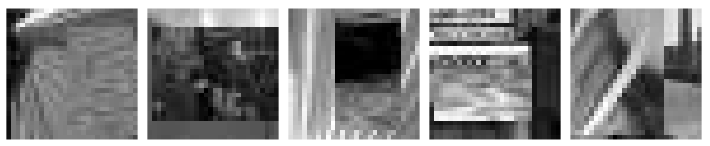
\includegraphics[scale=0.55]{figures/rect_image}
  \caption{sample images from \textit{rectangles-image} dataset.}
  \label{chap2_rect}
\end{figure}

\subsection{Results and Analysis}
\renewcommand{\arraystretch}{2.1}
\begin{table*}
\centering
\begin{tabular}{|c|c|c|c|c|c|c|c|}
  \hline
  \multirow{2}{*}{\textbf{Dataset}} & \multicolumn{7}{ |c| }{\textbf{Loss in Percentage}} \\
  \cline{2-8}
  & $\textrm{SVM}_{\textrm{RBF}}$ & $\textrm{SVM}_{\textrm{Poly}}$ & NNet & DBN-3 & SAA-3 & DBN-1 & MKMs\\
  \hline  
  \textit{back-rand} & 14.58 & 16.62 & 20.04 & \textbf{6.73} & 11.28 & 9.80 & 10.55\\
  \hline
  \textit{back-image} & 22.61 & 24.01 & 27.41 & 16.31 & 23.00 & \textbf{16.15} & 21.39\\
  \hline
  \textit{rot-back-image} & 55.18 & 56.41 & 62.16 & \textbf{47.39} & 51.93 & 52.21 & 51.61\\
  \hline
  \textit{rect-image} & 24.04 & 24.05 & 33.20 & 23.69 & 24.05 & \textbf{22.50} & 23.01\\
  \hline
\end{tabular}
\caption{Experimental Results of MKMs with Arc-cosine Kernels}
\label{tab_results_mkm}
\end{table*}
\renewcommand{\arraystretch}{1}

Table \ref{tab_results_mkm} also contains best results obtained from other models(\cite{dbn} et al.) like SVM with RBF kernel($\textrm{SVM}_{\textrm{RBF}}$), SVM with polynomial kenel($\textrm{SVM}_{\textrm{Poly}}$), single hidden layer feed-forward neural network(NNet\nomenclature{NNet}{Neural Network with one hidden layer}), Deep Belif Networks(DBN)\nomenclature{DBN}{Deep Belif Networks} with 1 hidden layer(DBN-1), DBN with 3 hidden layer(DBN-3) and 3 hidden layer Stacked Autoassociator Network(SAA-3). The first three models comes under shallow architectures and the remaining are deep architectures. From the table, it can be observed that MKMs outperforms all the remaining models except Deep Belif Networks(DBN). Compared to DBN the architecture, parameter tuning and optimization  are fairly simple in MKMs.

The change in the performance of the classifier when each adding layer to the model was also analyzed. Figures \ref{mkm_rand} and \ref{mkm_image} shows the variations in the classifier performance when model complexity was increased by adding more layers(on \textit{mnist-back-rand} and \textit{mnist-back-image} datasets respectively). The results indicates that in some cases better representation can be obtained even with a less complex model (eg: in case of \textit{mnist-back-image} dataset, where the performance degrades when model complexity increases).


\begin{figure}
  \centering
  \captionsetup{justification=centering,margin=0.1cm}
  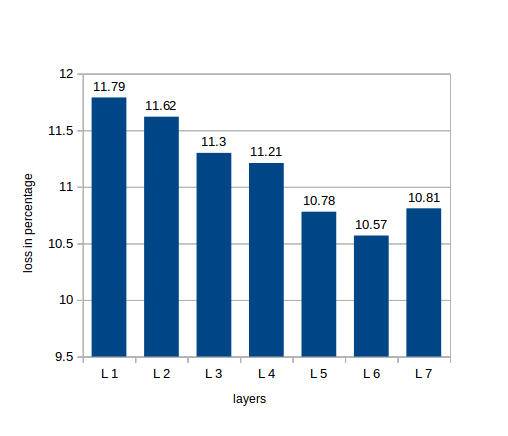
\includegraphics[scale=0.65]{figures/mkm_rand}
  \caption{Change in classifier performance on \textit{mnist-back-rand} dataset when increasing the number of layers.}
  \label{mkm_rand}
\end{figure}

\begin{figure}
  \centering
  \captionsetup{justification=centering,margin=0.1cm}
  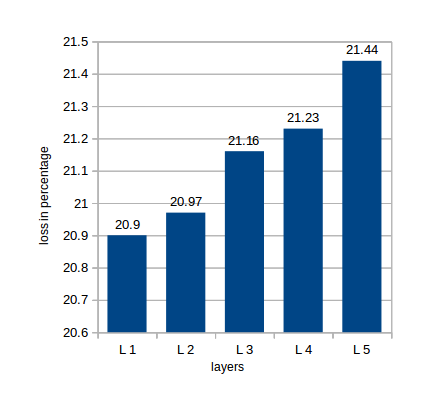
\includegraphics[scale=0.65]{figures/mkm_image}
  \caption{Change in classifier performance on \textit{mnist-back-image} dataset when increasing the number of layers.}
  \label{mkm_image}
\end{figure}

\section{Visualizing Features using tSNE}
\label{chap2_tsne}
In order to visualize the features learned by the MKM, t-distributed Stochastic Neighbor Embedding(tSNE, proposed by \cite{tsne} et al.) was used. tSNE\nomenclature{tSNE}{t-distributed Stochastic Neighbur Embedding} is a tool for visualizing high-dimensional data. It converts the similarities between datapoints to joint probabilities and tries to minimize the Kullback-Leibler divergence(KL divergence) between the joint probabilities of the low-dimensional embedding and the high dimensional data(\cite{tsne} et al.). tSNE is a variant of stochastic neighbor embedding \nomenclature{SNE}, that is much easier to optimize and produce significantly better visualizations by reducing the tendency of the  points to get accumulated  at the center of the map.

Suppose $X = \{x_1, x_2, \ldots, x_n\}$ are the high-dimensional datapoints, and $Y = \{y_1, y_2, \ldots, y_n\}$ the corresponding low-dimensional map points. In SNE, we first convert high-dimensional representation of datapoints into pairwise similarities that can be interpreted as conditional probabilities. Intuitively, the similarity of a datapoint $x_i$ to $x_j$ is interpreted as the probability of $x_i$ picking up $x_j$ as its neighbor with a Gaussian centered at $x_i$(denoted as $p_{j/i}$). Mathematically this is formulated as
\[ p_{j/i} = \frac{exp(-\norm{x_i-x_j}^2/2 \sigma_i^2}{\sum_{k\neq i} exp(-\norm{x_i - x_k}^2/2 \sigma_i^2)}  \]

where $\sigma_i$ is the variance of the Gaussian centered at $x_i$. For every $x_i$ we calculate corresponding $\sigma_i$ which will vary according to the density of datapoints around $x_i$(if the region around $x_i$ is dense $\sigma_i$ will be low and vice versa).

Similarly for the low-dimensional representations $y_i$ and $y_j$ corresponding to $x_i$ and $x_j$ respectively, we compute the conditional probability(denoted as $q_{j/i}$) by setting the variance of the Gaussian to $\frac{1}{\sqrt{2}}$. Thus
\[ q_{j/i} = \frac{exp(-\norm{y_i-y_j}^2}{\sum_{k\neq i} exp(-\norm{y_i - y_k}^2)}  \]

Since we are only interested in modelling pairwise similarity, we set $p_{i/i} = q_{i/i} = 0$. The crux of SNE as stated by \cite{tsne} et al. is ``if the map points $y_i$ and $y_j$ correctly model the similarity between high-dimensional datapoints $x_i$ and $x_j$ then the conditional probabilities $p_{j/i}$ and $q_{j/i}$ will be equal''. In this case, the cost function can be formulated to minimize the difference between conditional probabilities $p_{j/i}$ and $q_{j/i}$ using KL divergence. The cost function $C$ is defined as
\begin{equation}
C = \sum_{i}\textrm{KL}(\textrm{P}_i \big|\big| \textrm{Q}_i) = \sum_{i}\sum_{j} p_{j/i} log \frac{p_{j/i}}{q_{j/i}}
\label{cost_tsne}
\end{equation}
where $\textrm{P}_i$ is the conditional probability distribution over all other datapoints given datapoint $x_i$ and $\textrm{Q}_i$ is the conditional probability distribution over all other map points given the map point $y_i$.

The minimization of the cost function in \ref{cost_tsne} is performed by using gradient descent method. The gradient is computed as
\[ \frac{\partial C}{\partial y_i} = 2\sum_j(p_{j/i}-q_{j/i} + p_{i/j}-q_{i/j})(y_i - y_j) \]
Though SNE can produce good quality visualizations, it has the following limitations.
\begin{itemize}
\item Since the KL divergence is not symmetric, different types of error in the pairwise distances in low-dimensional map are not weighted equally(there is a large cost for using widely separated map points to represent nearby datapoints, but the cost is small for using nearby map points to represent widely separated datapoints).
\item crowding of map points in the center of the map.
\end{itemize}

tSNE is a variant of SNE which improves the visualization quality by alleviating the above mentioned problems.
\begin{itemize}
\item It uses a symmetric version of the SNE cost function by employing a joint probability distribution instead of the conditional probability distribution used by SNE. This also results in simpler gradients.
\item It uses student-t distribution to compute the similarity between map points. tSNE employs a heavy-tailed distribution for the map points to alleviate both the crowding problem and optimization problems of SNE.
\end{itemize}

In the symmetric version of the  tSNE the cost function is computed as shown below.
\begin{equation*}
C = \textrm{KL}(\textrm{P} \big|\big| \textrm{Q}) = \sum_{i}\sum_{j} p_{ij} log \frac{p_{ij}}{q_{ij}}
\end{equation*}
where $P$ and $Q$ are the joint probability distribution functions in the high-dimensional and low-dimensional space respectively. Here also we set $p_{ii}$ and $q_{ii}$ to zero. The symmetry in the cost function is achieved due to the fact that $p_{ij} = p_{ji}$ and $q_{ij} = q_{ji}$ $\forall i,j$. The joint probability in high-dimensional space($p_{ij}$) and low-dimensional space($q_{ij}$) are computed as
\[ p_{ij} = \frac{exp(-\norm{x_i-x_j}^2/2 \sigma^2}{\sum_{k\neq l} exp(-\norm{x_k - x_l}^2/2 \sigma^2)}  \]
\[ q_{ij} = \frac{exp(-\norm{y_i-y_j}^2}{\sum_{k\neq l} exp(-\norm{y_k - y_l}^2)}  \]
The gradient of the symmetric SNE has a fairly simple form
\[ \frac{\partial C}{\partial y_i} = 4\sum_j(p_{ij}-q_{ij})(y_i - y_j) \]
Symmetric SNE still faces problems when a datapoint $x_i$ is an outlier; when $x_i$ is an outlier $\norm{x_i-x_j}^2$ is large for all $x_j$ with $x_i$, hence $p_{ij}$ are extremely low, so the location of its low-dimensional map point $y_i$ has very little effect on the cost function. This problem is addressed in tSNE by defining $p_{ij} = \frac{p_{j/i} + p_{i/j}}{2n}$, which ensures that $\sum_j p_{ij} \ge \frac{1}{2n}$ $\forall \textrm{ } x_i$, hence each datapoint $x_i$ makes a significant contribution to the cost function. The crowding problem is addressed in tSNE by using a student t-distribution with one degree of freedom as the heavy-tailed distribution in the low-dimensional map. Thus the joint probability $q_{ij}$ is computed as
\[ q_{ij} = \frac{(1+\norm{y_i-y_j}^2)^-1}{\sum_{k \neq l} (1+\norm{y_k-y_l}^2)^-1} \] 
Then, finally the gradient of the cost function is obtained as
\[ \frac{\partial C}{\partial y_i} = 4\sum_j(p_{ij}-q_{ij})(y_i - y_j)(1+\norm{y_i-y_j}^2)^-1) \]

tSNE was employed in our experiments to understand the changes in the data distribution before and after the feature learning process. Figure \ref{tsne_rand_raw} shows the tSNE embedding of the raw data from \textit{mnist-back-rand} dataset and figure \ref{tsne_rand_mkm} shows the same embedding applied on the features produced by MKM with arc-cosine kernels. The tSNE embedding of features learned by MKMs are crowded near the center, hence it was difficult to interpret the separability.

\begin{sidewaysfigure}
  \centering
  \captionsetup{justification=centering,margin=0.1cm}
  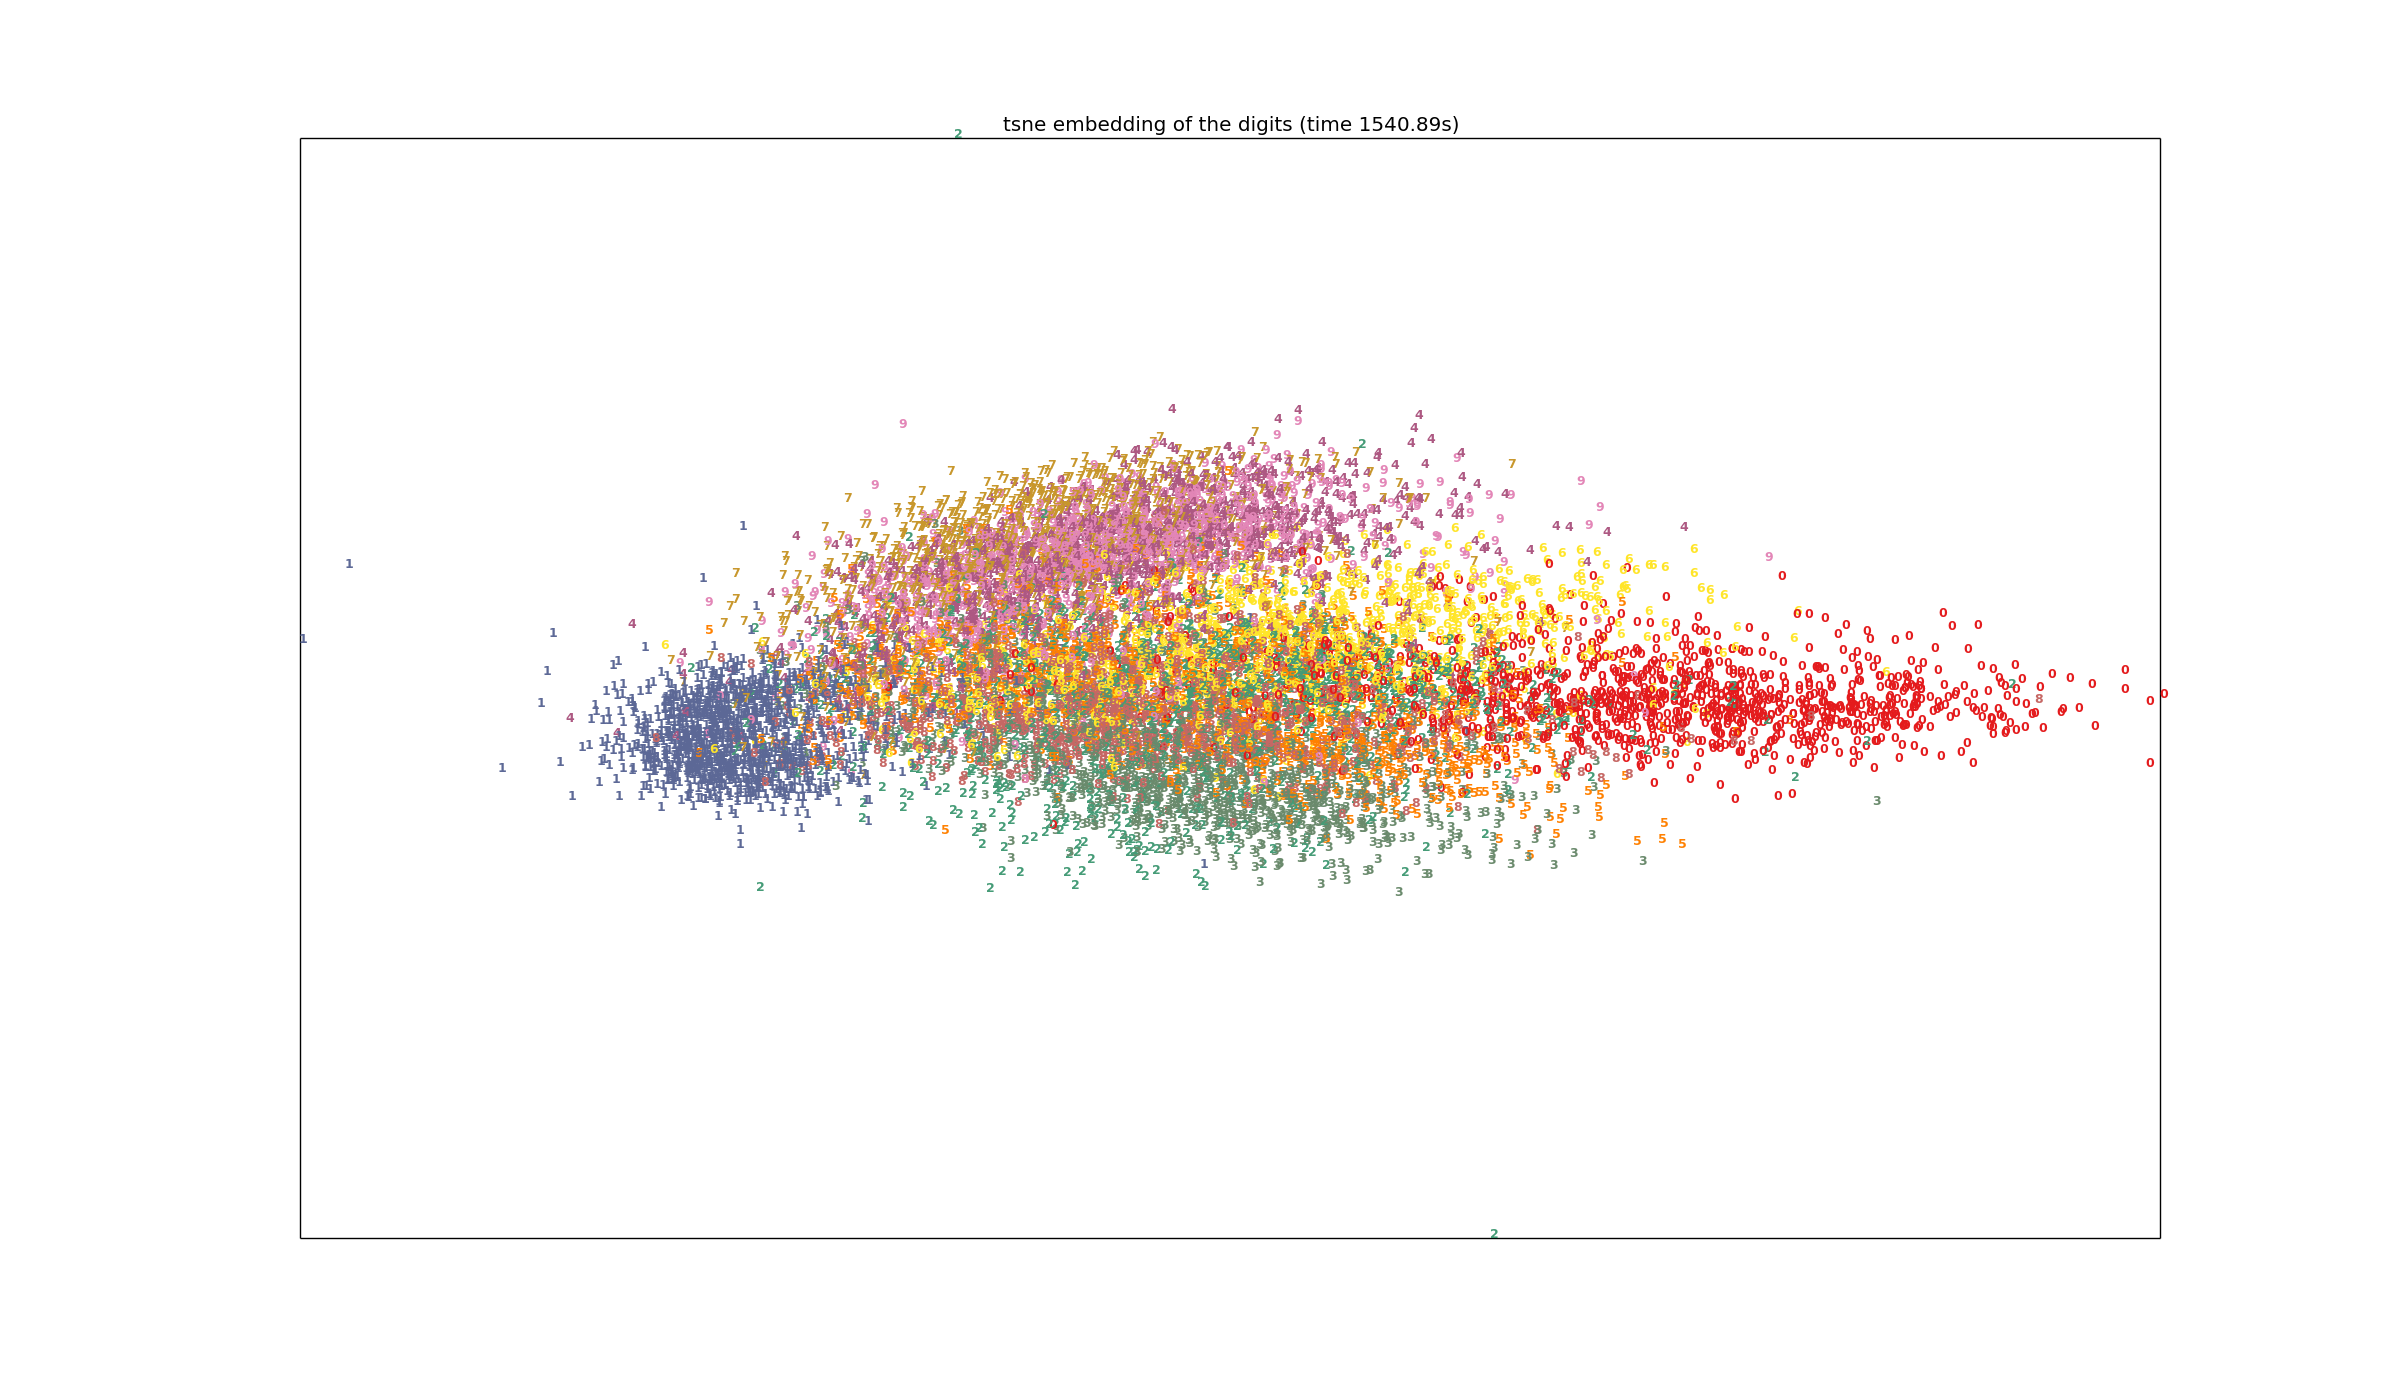
\includegraphics[scale=0.45]{figures/tsne_rand_rawdata}
  \caption{tSNE embedding of raw data from \textit{mnist-back-rand} dataset.}
  \label{tsne_rand_raw}
\end{sidewaysfigure}


\begin{sidewaysfigure}
  \centering
  \captionsetup{justification=centering,margin=0.1cm}
  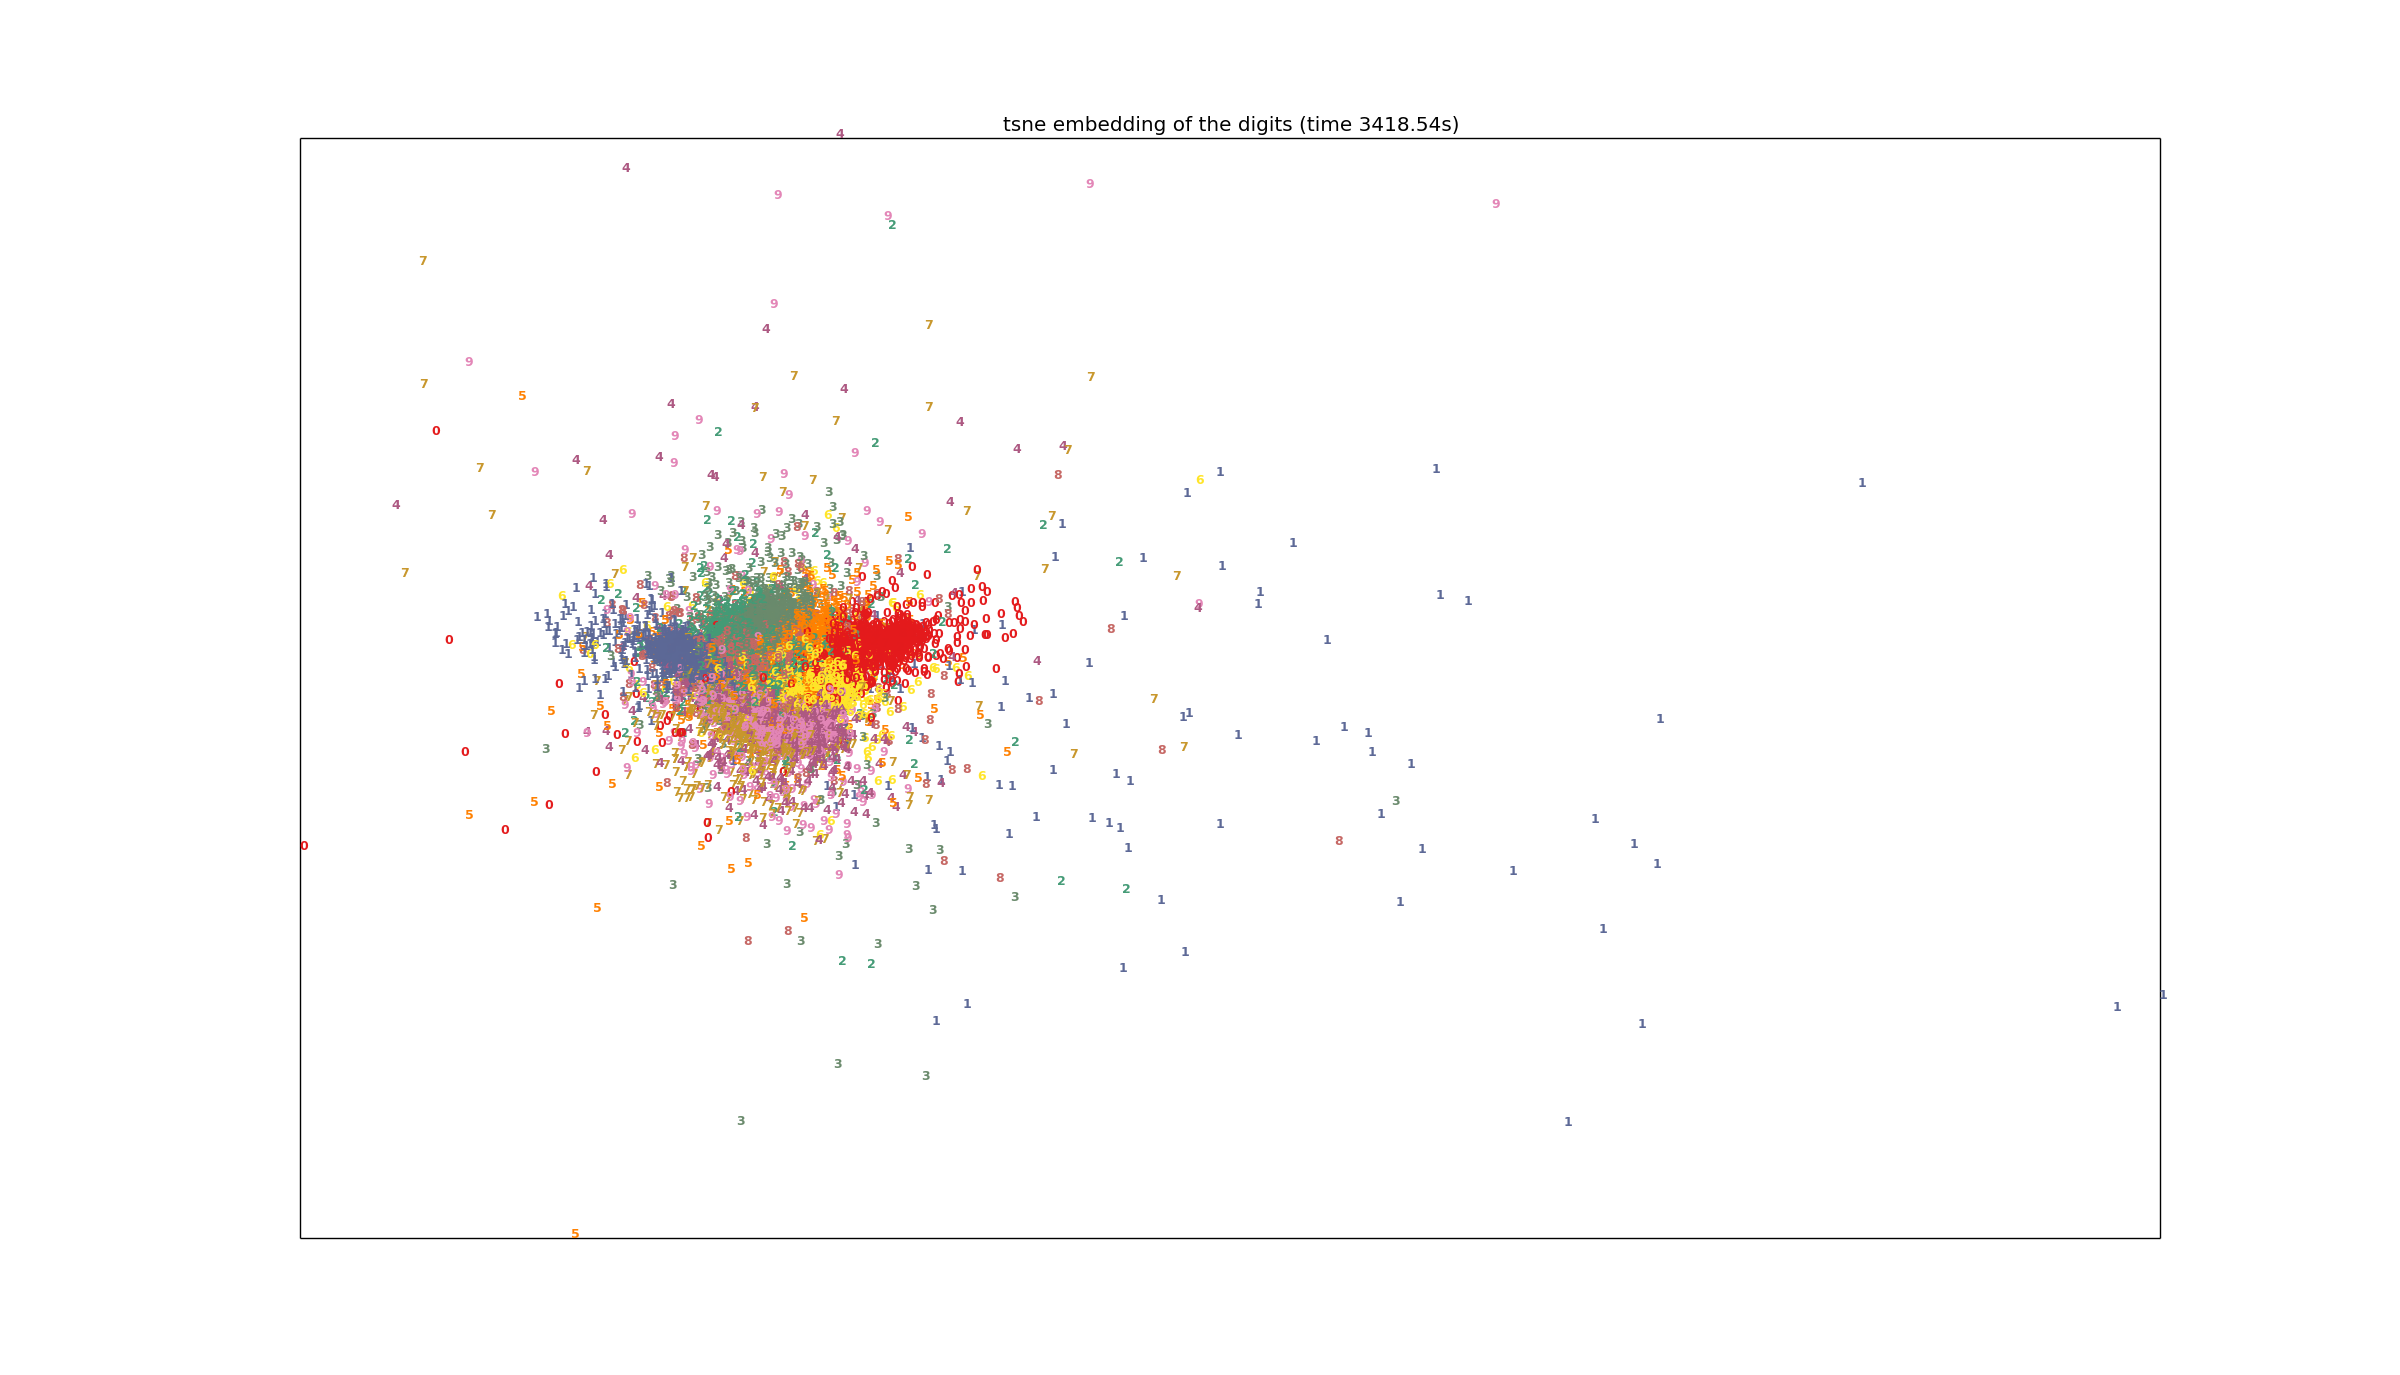
\includegraphics[scale=0.45]{figures/tsne_rand_mkmbest}
  \caption{tSNE embedding of features obtained by MKM from \textit{mnist-back-rand} dataset.}
  \label{tsne_rand_mkm}
\end{sidewaysfigure}



\section{MKMs with Mixed Kernels}
\label{chap2_mkm_mix}
We tried different kernel functions in different layers of MKMs (Gaussian, arc-cosine, polynomial etc.) while performing KPCA. It had been seen that mixing a layer of Gaussian or polynomial kernel in between successive layers of arc-cosine kernel improves the result. This further supported the belief that, with more similarity information (by using more kernels) in hand, we can build better representations. Table \ref{tab_results_mix} shows the result obtained with the mixed kernel models. Because of the improved performance, we used  Multi-layer Multiple Kernel Machines(ML-MKL) model for our analysis, whose  discussion is given in the next chapter.

\renewcommand{\arraystretch}{2.1}
\begin{table}
\centering
\begin{tabular}{|c|c|c|c|c|c|c|c|}
  \hline
  \multirow{2}{*}{\textbf{Dataset}} & \multicolumn{7}{ |c| }{\textbf{Loss in Percentage}} \\
  \cline{2-8}
  & $\textrm{SVM}_{\textrm{RBF}}$ & $\textrm{SVM}_{\textrm{Poly}}$ & NNet & DBN-3 & SAA-3 & DBN-1 & $\textrm{MKMs}_\textrm{(mix)}$\\
  \hline  
  \textit{back-rand} & 14.58 & 16.62 & 20.04 & \textbf{6.73} & 11.28 & 9.80 & 9.54\\
  \hline
  \textit{back-image} & 22.61 & 24.01 & 27.41 & 16.31 & 23.00 & \textbf{16.15} & 20.94\\
  \hline
  \textit{rot-back-image} & 55.18 & 56.41 & 62.16 & \textbf{47.39} & 51.93 & 52.21 & 54.03\\
  \hline
  \textit{rect-image} & 24.04 & 24.05 & 33.20 & 23.69 & 24.05 & \textbf{22.50} & 25.04\\
  \hline
\end{tabular}
\caption{Experimental Results of MKMs with Mixed Kernels}
\label{tab_results_mix}
\end{table}
\renewcommand{\arraystretch}{1}

As in MKMs with arc-cosine kernel, we chose top 5 percent features based on univariate test score for the mixed kernel MKMs. The classifier used in the output layer was an SVM\nomenclature{SVM}{Support Vector Machines} with arc-cosine kernel. The results indicates that MKMs with mixed kernels improved the classifier performance for \textit{mnist-back-rand} and \textit{mnist-back-image} datasets, whereas the classification accuracy declined in the case of \textit{mnist-rot-back-image} and \textit{rectangles-image} dataset. The tSNE embedding of the features produced by MKMs with mixed kernels is shown in figure \ref{tsne_rand_mkmmix} (for \textit{mnist-back-rand} dataset). The best result in this dataset was obtained from a model consisting of three layers with a Gaussian kernel in the middle layer. The visualization indicates that, MKMs with mixed kernels has good separability between different classes.
\begin{sidewaysfigure}
  \centering
  \captionsetup{justification=centering,margin=0.1cm}
  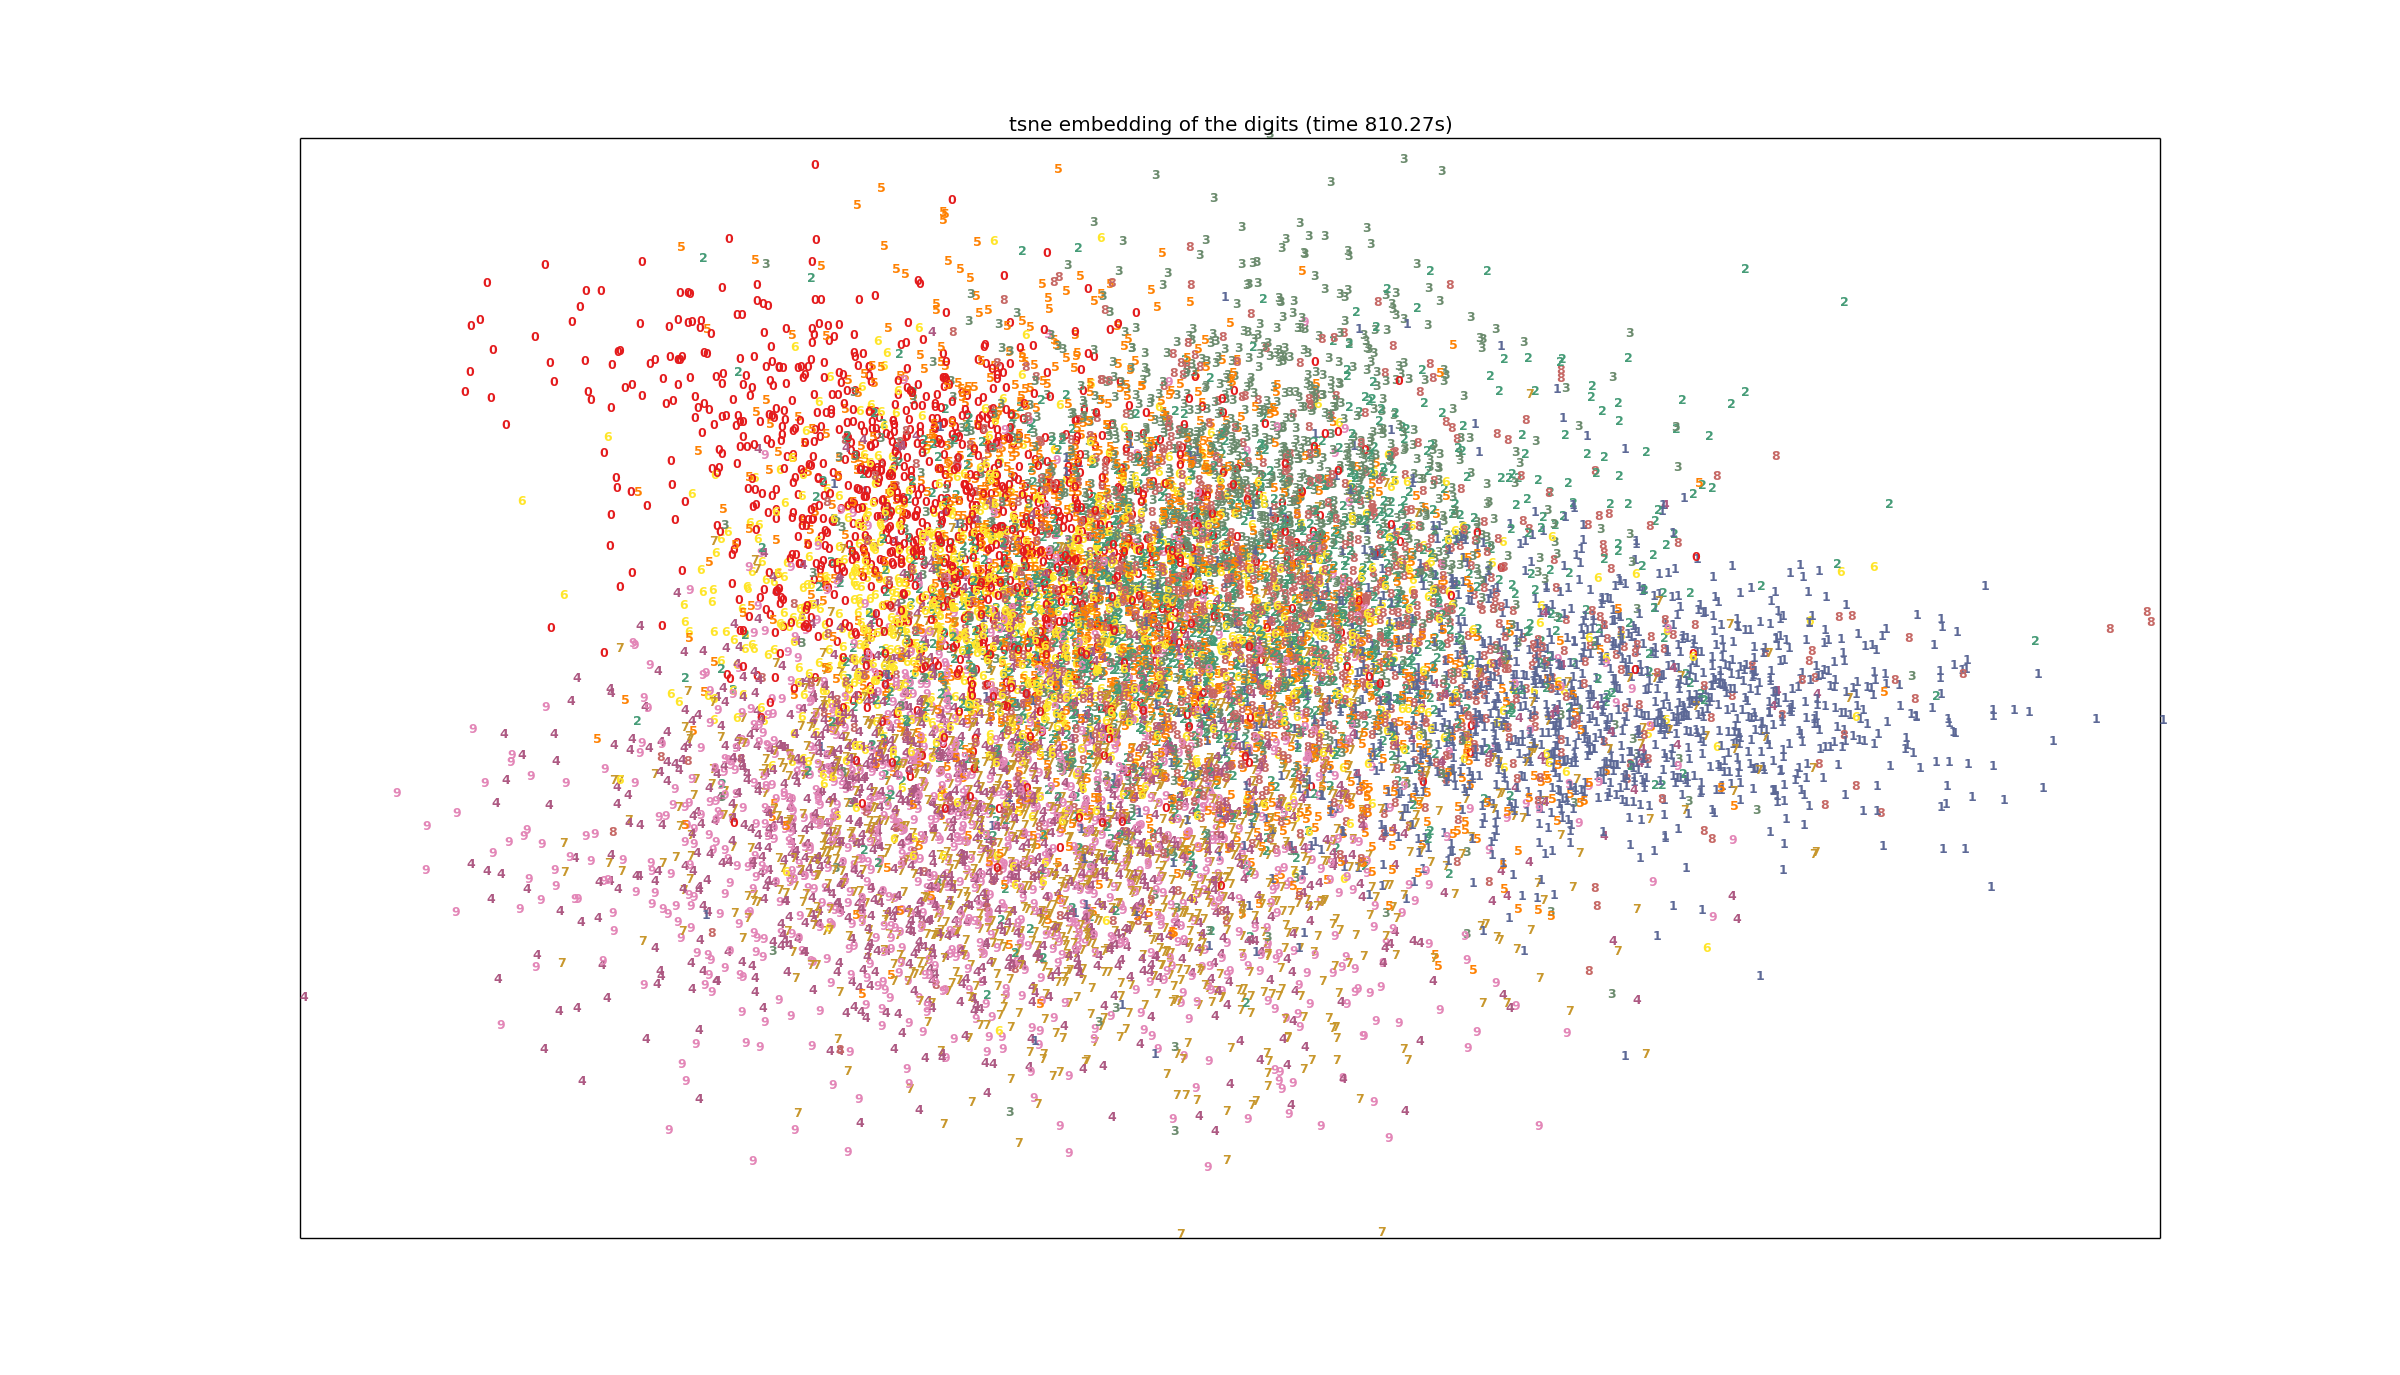
\includegraphics[scale=0.45]{figures/tsne_rand_mkmmix}
  \caption{tSNE embedding of features obtained by MKM with mixed kernels from \textit{mnist-back-rand} dataset.}
  \label{tsne_rand_mkmmix}
\end{sidewaysfigure}


\section{Conclusion}
\label{chap2_conc}
In this chapter we analysed the MKMs framework which has the characteristics of deep learning algorithms by employing  kernel methods. The empirical study indicated that MKMs are performing comparable with that of  popular deep learning algorithms like DBN, SAA etc. We also analysed the performnace of MKMs with mixed kernels. The mixing produces better results when other kernels are sandwiched between two arc-cosine kernels.

The visualization of features learned by MKMs are difficult to interpret due to crowding of datapoints near the center, but for MKMs with mixed kernels the visualization indicates that the separation is good enough between different classes, even though the samples from same class is distributed in different locations.
